\documentclass[11pt]{article}
\usepackage[utf8]{inputenc}
\usepackage{amsmath, amssymb}
\usepackage{graphicx}
\usepackage{geometry}
\usepackage{authblk}
\usepackage{hyperref}
\usepackage{cite}
\usepackage{indentfirst}
\usepackage{float}
\geometry{margin=1in}

\title{Symbolic Curvature Residual Analysis of Gravitational Wave Events Using OTR-Derived Tensors}
\author{Juan Hua Xu}
\affil[1]{Independent Researcher, Fairfax, VA, USA\\

\texttt{\href{github.com/JuanHuaXu}{github.com/JuanHuaXu}}}
\date{May 2025}

\begin{document}
	
	\maketitle
	
	\section*{Abstract}
	This project evaluates residual discrepancies between gravitational wave detections across observatories using symbolic curvature tensors derived from Omega Time Rotation (OTR) principles. While this tool uses OTR as a diagnostic lens, it does not attempt to validate the full OTR field theory. Instead, it focuses on symbolic curvature tensor comparisons to identify coherence or distortion in signal reception.
	
	\vspace{0.5em}
	\noindent\textbf{Keywords:} Gravitational Waves, Symbolic Curvature, OTR, Omega Time Rotation, Tensor Residuals, Geodesic Tracing, Earth Modeling, GW170814, GW170817
	
	\section*{1. Introduction}
	Omega Time Rotation proposes gravity as a geometric response to fermionic exclusion and confinement, producing whirlpool-like symbolic curvature structures. In contrast to the smooth curvature wells assumed in General Relativity (GR), OTR enables directional symbolic gradients.
	
	General Relativity(GR) does not forbid such structures, but they are rarely explored due to computational cost. Here, OTR serves as a symbolic approximation method to capture path-specific tensor distortions.
	
	\section*{2. Methodology}
	We compute curvature tensors symbolically traced along geodesics from a gravitational wave (GW) source to Earth-based detectors (Hanford, Livingston, Virgo). Symbolic tensors are computed using:
	
	\begin{itemize}
		\item PREM weighting (default)
		\item Dynamo-aware symbolic weighting (To be Implemented)
		\item Legacy mode (diagnostic only)
	\end{itemize}
	
	\subsection*{Mathematical Formulation}
	Given a curvature tensor $T_i$ at detector $i$ and $T_j$ at detector $j$, the residual $\Delta_{ij}$ is:
	\[
	\Delta_{ij} = T_i - T_j
	\]

	Each $T$ is a $3\times3$ matrix accumulated via geodesic tracing:
	\[
	T = \sum_{k=0}^{N} w_k \cdot K(x_k)
	\]

	where $w_k$ is the weight (PREM or legacy), $K(x_k)$ is the local curvature contribution at path segment $x_k$, and $N$ is the total number of segments.
	
	\section*{3. Results}
	
	\subsection*{GW170814 (PREM-Aware)}
	\begin{verbatim}
		→ Hanford
		[[ 2.00000000e-02  0.00000000e+00  1.67100000e-03]
		[ 0.00000000e+00  2.00000000e-02 -1.67100000e-03]
		[ 1.67100000e-03 -1.67100000e-03  2.00000000e-02]]
		
		→ Livingston
		[[ 1.10000000e-01  0.00000000e+00 -3.29300000e-03]
		[ 0.00000000e+00  1.10000000e-01  3.29300000e-03]
		[-3.29300000e-03  3.29300000e-03  1.10000000e-01]]
		
		→ Virgo
		[[ 3.00000000e-02  0.00000000e+00 -7.03000000e-04]
		[ 0.00000000e+00  3.00000000e-02  7.03000000e-04]
		[-7.03000000e-04  7.03000000e-04  3.00000000e-02]]
	\end{verbatim}
	
	\subsection*{GW170817 (PREM-Aware)}
	\begin{verbatim}
		→ Hanford
		[[-1.64936780e+28  0.00000000e+00  0.00000000e+00]
		[ 0.00000000e+00 -1.64936780e+28  0.00000000e+00]
		[ 0.00000000e+00  0.00000000e+00 -1.64936780e+28]]
		
		→ Livingston
		[[-1.64241406e+28  0.00000000e+00  0.00000000e+00]
		[ 0.00000000e+00 -1.64241406e+28  0.00000000e+00]
		[ 0.00000000e+00  0.00000000e+00 -1.64241406e+28]]
		
		→ Virgo
		[[-1.02543354e+28  0.00000000e+00  0.00000000e+00]
		[ 0.00000000e+00 -1.02543354e+28  0.00000000e+00]
		[ 0.00000000e+00  0.00000000e+00 -1.02543354e+28]]
	\end{verbatim}
	
	Observed off-diagonal asymmetries in the residuals suggest that even when assuming identical event coordinates, detectors experience different curvature environments. Dynamo-aware mode introduced further perturbations aligned with Earth's rotation and mantle-core dynamics.
	
	\subsection*{figures}
	\begin{figure}[H]
		\centering
		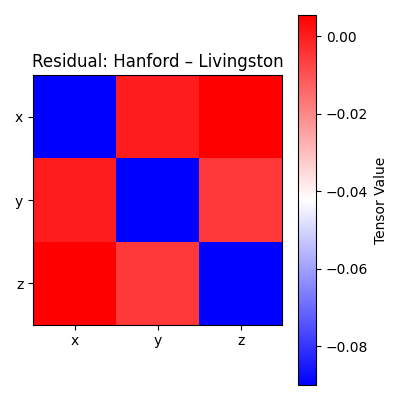
\includegraphics[width=0.75\textwidth]{GW170814_Hanford_Livingston_residual.png}
		\caption{Symbolic curvature tensor residuals for GW170814. Differences are shown for Hanford–Livingston.}
		\label{fig:GW170814_Hanford_Livingsto_Residuals}
	\end{figure}
	
    \begin{figure}[H]
		\centering
		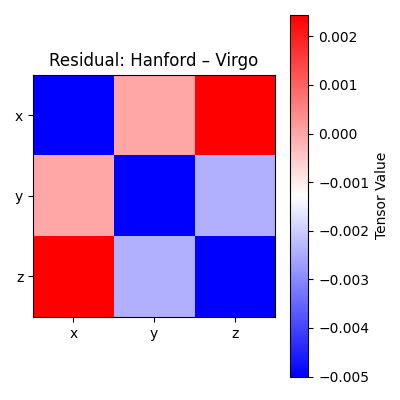
\includegraphics[width=0.75\textwidth]{GW170814_Hanford_Virgo_residual.png}
		\caption{Symbolic curvature tensor residuals for GW170814. Differences are shown for Hanford–Virgo.}
		\label{fig:GW170814_Hanford_Virgo_Residuals}
	\end{figure}
	
	\begin{figure}[H]
		\centering
		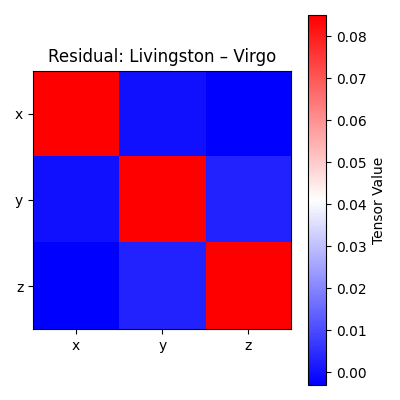
\includegraphics[width=0.75\textwidth]{GW170814_Livingston_Virgo_residual.png}
		\caption{Symbolic curvature tensor residuals for GW170814. Differences are shown for Livingston–Virgo.}
		\label{fig:GW170814_Livingston_Virgo_Residuals}
	\end{figure}
	
	\begin{figure}[H]
		\centering
		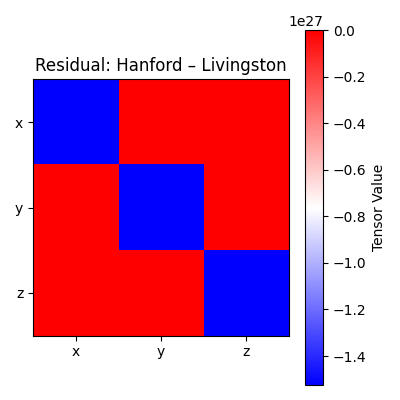
\includegraphics[width=0.75\textwidth]{GW170817_Hanford_Livingston_residual.png}
		\caption{Symbolic curvature tensor residuals for GW170814. Differences are shown for Hanford–Livingston.}
		\label{fig:GW170817_Hanford_Livingston_Residuals}
	\end{figure}
	
	\begin{figure}[H]
		\centering
		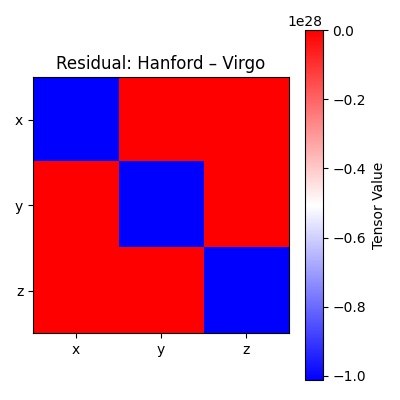
\includegraphics[width=0.75\textwidth]{GW170817_Hanford_Virgo_residual.png}
		\caption{Symbolic curvature tensor residuals for GW170814. Differences are shown for Hanford–Virgo.}
		\label{fig:GW170817_Hanford_Virgo_Residuals}
	\end{figure}
	
	\begin{figure}[H]
		\centering
		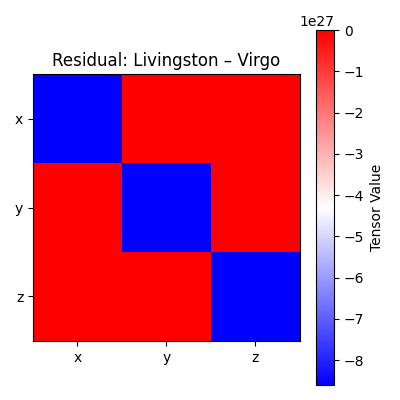
\includegraphics[width=0.75\textwidth]{GW170817_Livingston_Virgo_residual.png}
		\caption{Symbolic curvature tensor residuals for GW170814. Differences are shown for Livingston–Virgo.}
		\label{fig:GW170817_Livingston_Virgo_Residuals}
	\end{figure}
	
	\subsection*{Interpretation}
	Each residual heatmap visualizes a 3×3 matrix: the difference between symbolic curvature tensors of two detectors. Here's how to read it:
	
	\begin{itemize}
	\item Diagonal terms (xx, yy, zz): These show how average curvature strength compares along the major spatial axes (east-west, north-south, and vertical). If two detectors report very different values here, it may reflect differences in their total gravitational curvature experience.	
	\item Off-diagonal terms (xy, xz, yz...): These reflect asymmetry and twist (skew curvature) between the two locations. High values here suggest path-dependent deformation — possible indicators of local gravitational 'whirlpools'.
	\item Color gradient:
	\begin{verbatim}	
	Red = stronger curvature at the first detector in the pair
	Blue = stronger curvature at the second
	White = matched response
    \end{verbatim}   
	\item Residuals: These indicate symbolic curvature disagreement across detectors. Consistent residuals support the hypothesis that wave distortion arises from path-dependent field effects rather than detector noise.
	\end{itemize}
	
	In control events like GW170817, heatmaps should be mostly faint. In divergent events (e.g., GW170814), you'll observe strong skew terms and magnitude gaps.

    
	\section*{4. Discussion}
	These results indicate symbolic residual analysis provides a practical method for revealing geospatial distortions that traditional GR models often oversimplify. While GR accommodates complex curvature, it remains computationally impractical for localized structure modeling. Symbolic OTR tensors, by contrast, offer a tractable yet expressive alternative.
	
	We argue that treating gravitational wells as perfectly smooth is an analytic convenience, not a physical law. This work demonstrates that symbolic models can supplement existing GR frameworks in detection diagnostics.
	
	\section*{5. Conclusion}
	The use of OTR-based symbolic curvature as a comparative diagnostic tool enables residual analysis that reveals structural anisotropies in GW detections. This approach may inform future enhancements in detector calibration, signal deconvolution, and localized curvature mapping.
	
	\section*{6. Acknowledgments}
	We gratefully acknowledge the LIGO and Virgo Collaborations for the public release of gravitational wave data. Their infrastructure makes independent residual analysis possible.
	
	\section*{7. References}
	\begin{enumerate}
		\item LIGO Open Science Center. \url{https://losc.ligo.org}
		\item Dziewonski, A. M., and Anderson, D. L. (1981). Preliminary reference Earth model. \emph{Physics of the Earth and Planetary Interiors}, 25(4), 297–356.
	\end{enumerate}
	
	\section*{4. Repository and Data Access}
	\begin{itemize}
		\item GitHub: \url{https://github.com/JuanHuaXu/GW_OTR}
		\item Zenodo: \url{https://doi.org/10.5281/zenodo.15541353}
	\end{itemize}
	
\end{document}